\setcounter{section}{2}
\section{Teilversuch 3: Strömung einer Flüssigkeit durch eine Kapillare}
	Fehler bei jeder Messung der Höhe $h = \SI{1}{\milli\meter}$\\
	Fehler bei jeder Messung der Zeit $t = \SI{0.2}{\second}$ 

	Die höhe $h_\infty = \SI{83(2)}{\milli\meter}$ 

	\begin{center}
		\begin{tabular}{l *{8}{r}}
			\toprule
			$t / \si{\minute}$ & \num{0} & \num{1} & \num{2} & \num{3} & \num{4} & \num{5} & \num{6} & \num{7}  \\
			\midrule
			$h / \si{\milli\meter}$ & \num{418} & \num{386} & \num{358} & \num{333} & \num{311} & \num{290} & \num{271} & \num{254} \\
			$\ln\left[\left(h - h_\infty\right) / \si{\milli\meter}\right]$ &\num{5.81} & \num{5.71} & \num{5.62} & \num{5.52} & \num{5.43} & \num{5.33} & \num{5.24} & \num{5.14} \\
			\bottomrule \\
			\toprule
			$t / \si{\minute}$ & \num{8} & \num{9} & \num{10} & \num{11} & \num{12} & \num{13} & \num{14} & \num{15} \\
			\midrule 
			$h / \si{\milli\meter}$ & \num{238} & \num{225} & \num{212} & \num{200} & \num{190} & \num{180} & \num{172} & \num{164} \\
			$\ln\left[\left(h - h_\infty\right) / \si{\milli\meter}\right]$ & \num{5.04} & \num{4.96} & \num{4.86} & \num{4.76} & \num{4.67} & \num{4.57} & \num{4.49} & \num{4.39} \\
			\bottomrule
		\end{tabular}
	\end{center}

	Fehler bei jeder Rechnung von $y =\ln\left[\left(h - h_\infty\right) / \si{\milli\meter}\right]$ ist gegeben durch:
	\begin{equation}
		\Delta y = \gausserror{L}{h, h_\infty} = \frac{1}{h-h_\infty} \sqrt{\left(\SI{1}{\milli\meter}\right)^2 + \left(\SI{2}{\milli\meter}\right)^2} = \frac{\sqrt{5}~\si{\milli\meter}}{h-h_\infty}
	\end{equation}

	Normale Anpassungsalgorithmen (Methode der kleinsten Quadrate) setzen voraus, dass die $x$-Variable die unabhängige Variable ist und als fehlerfrei genommen werden kann. Da es sich bei diesem Versuch um zwei gemessene Variablen handelt, gibt es bei beiden Variablen $y$ und $t$ Fehler. Die Fehler müssen dann während der Kurvenanpassung berücksichtigt werden. 

	Aus Gleichung (6) der Anleitung haben wir den folgenden Zusammenhang:
	\begin{equation}
		\ln\left(h-h_\infty\right) = -\frac{\pi r^4 \rho g}{8\eta L A_v}t + \ln\left(h_0-h_\infty\right) \equiv \alpha t + \beta \label{eqn:tv3main}
	\end{equation}

    \newpage
	Die Daten wurden dann mit \gnuplot{} geplottet und es wurde eine Kurvenanpassung durchgeführt (Siehe Appendix \ref{appdx:gnuplotTV3}):

	\begin{figure}[H]
		\centering
		% GNUPLOT: LaTeX picture with Postscript
\begingroup
  \makeatletter
  \providecommand\color[2][]{%
    \GenericError{(gnuplot) \space\space\space\@spaces}{%
      Package color not loaded in conjunction with
      terminal option `colourtext'%
    }{See the gnuplot documentation for explanation.%
    }{Either use 'blacktext' in gnuplot or load the package
      color.sty in LaTeX.}%
    \renewcommand\color[2][]{}%
  }%
  \providecommand\includegraphics[2][]{%
    \GenericError{(gnuplot) \space\space\space\@spaces}{%
      Package graphicx or graphics not loaded%
    }{See the gnuplot documentation for explanation.%
    }{The gnuplot epslatex terminal needs graphicx.sty or graphics.sty.}%
    \renewcommand\includegraphics[2][]{}%
  }%
  \providecommand\rotatebox[2]{#2}%
  \@ifundefined{ifGPcolor}{%
    \newif\ifGPcolor
    \GPcolortrue
  }{}%
  \@ifundefined{ifGPblacktext}{%
    \newif\ifGPblacktext
    \GPblacktexttrue
  }{}%
  % define a \g@addto@macro without @ in the name:
  \let\gplgaddtomacro\g@addto@macro
  % define empty templates for all commands taking text:
  \gdef\gplbacktext{}%
  \gdef\gplfronttext{}%
  \makeatother
  \ifGPblacktext
    % no textcolor at all
    \def\colorrgb#1{}%
    \def\colorgray#1{}%
  \else
    % gray or color?
    \ifGPcolor
      \def\colorrgb#1{\color[rgb]{#1}}%
      \def\colorgray#1{\color[gray]{#1}}%
      \expandafter\def\csname LTw\endcsname{\color{white}}%
      \expandafter\def\csname LTb\endcsname{\color{black}}%
      \expandafter\def\csname LTa\endcsname{\color{black}}%
      \expandafter\def\csname LT0\endcsname{\color[rgb]{1,0,0}}%
      \expandafter\def\csname LT1\endcsname{\color[rgb]{0,1,0}}%
      \expandafter\def\csname LT2\endcsname{\color[rgb]{0,0,1}}%
      \expandafter\def\csname LT3\endcsname{\color[rgb]{1,0,1}}%
      \expandafter\def\csname LT4\endcsname{\color[rgb]{0,1,1}}%
      \expandafter\def\csname LT5\endcsname{\color[rgb]{1,1,0}}%
      \expandafter\def\csname LT6\endcsname{\color[rgb]{0,0,0}}%
      \expandafter\def\csname LT7\endcsname{\color[rgb]{1,0.3,0}}%
      \expandafter\def\csname LT8\endcsname{\color[rgb]{0.5,0.5,0.5}}%
    \else
      % gray
      \def\colorrgb#1{\color{black}}%
      \def\colorgray#1{\color[gray]{#1}}%
      \expandafter\def\csname LTw\endcsname{\color{white}}%
      \expandafter\def\csname LTb\endcsname{\color{black}}%
      \expandafter\def\csname LTa\endcsname{\color{black}}%
      \expandafter\def\csname LT0\endcsname{\color{black}}%
      \expandafter\def\csname LT1\endcsname{\color{black}}%
      \expandafter\def\csname LT2\endcsname{\color{black}}%
      \expandafter\def\csname LT3\endcsname{\color{black}}%
      \expandafter\def\csname LT4\endcsname{\color{black}}%
      \expandafter\def\csname LT5\endcsname{\color{black}}%
      \expandafter\def\csname LT6\endcsname{\color{black}}%
      \expandafter\def\csname LT7\endcsname{\color{black}}%
      \expandafter\def\csname LT8\endcsname{\color{black}}%
    \fi
  \fi
    \setlength{\unitlength}{0.0500bp}%
    \ifx\gptboxheight\undefined%
      \newlength{\gptboxheight}%
      \newlength{\gptboxwidth}%
      \newsavebox{\gptboxtext}%
    \fi%
    \setlength{\fboxrule}{0.5pt}%
    \setlength{\fboxsep}{1pt}%
\begin{picture}(7200.00,5040.00)%
    \gplgaddtomacro\gplbacktext{%
      \csname LTb\endcsname%%
      \put(814,704){\makebox(0,0)[r]{\strut{}$4,2$}}%
      \put(814,1112){\makebox(0,0)[r]{\strut{}$4,4$}}%
      \put(814,1521){\makebox(0,0)[r]{\strut{}$4,6$}}%
      \put(814,1929){\makebox(0,0)[r]{\strut{}$4,8$}}%
      \put(814,2337){\makebox(0,0)[r]{\strut{}$5$}}%
      \put(814,2746){\makebox(0,0)[r]{\strut{}$5,2$}}%
      \put(814,3154){\makebox(0,0)[r]{\strut{}$5,4$}}%
      \put(814,3562){\makebox(0,0)[r]{\strut{}$5,6$}}%
      \put(814,3971){\makebox(0,0)[r]{\strut{}$5,8$}}%
      \put(814,4379){\makebox(0,0)[r]{\strut{}$6$}}%
      \put(946,484){\makebox(0,0){\strut{}$-100$}}%
      \put(1478,484){\makebox(0,0){\strut{}$0$}}%
      \put(2011,484){\makebox(0,0){\strut{}$100$}}%
      \put(2543,484){\makebox(0,0){\strut{}$200$}}%
      \put(3076,484){\makebox(0,0){\strut{}$300$}}%
      \put(3608,484){\makebox(0,0){\strut{}$400$}}%
      \put(4141,484){\makebox(0,0){\strut{}$500$}}%
      \put(4673,484){\makebox(0,0){\strut{}$600$}}%
      \put(5206,484){\makebox(0,0){\strut{}$700$}}%
      \put(5738,484){\makebox(0,0){\strut{}$800$}}%
      \put(6271,484){\makebox(0,0){\strut{}$900$}}%
      \put(6803,484){\makebox(0,0){\strut{}$1000$}}%
    }%
    \gplgaddtomacro\gplfronttext{%
      \csname LTb\endcsname%%
      \put(209,2541){\rotatebox{-270}{\makebox(0,0){\strut{}$\ln \left[\left(h - h_\infty\right) / \si{\milli\meter}\right]$}}}%
      \put(3874,154){\makebox(0,0){\strut{}Zeit $t$ ($\si{\second}$)}}%
      \put(3874,4709){\makebox(0,0){\strut{}Wasserstand beim Kapilarviskosimeter im Verlauf der Zeit}}%
      \csname LTb\endcsname%%
      \put(5816,4206){\makebox(0,0)[r]{\strut{}$-0,00158x + 5,80951$}}%
      \csname LTb\endcsname%%
      \put(5816,3986){\makebox(0,0)[r]{\strut{}tv3.dat}}%
    }%
    \gplbacktext
    \put(0,0){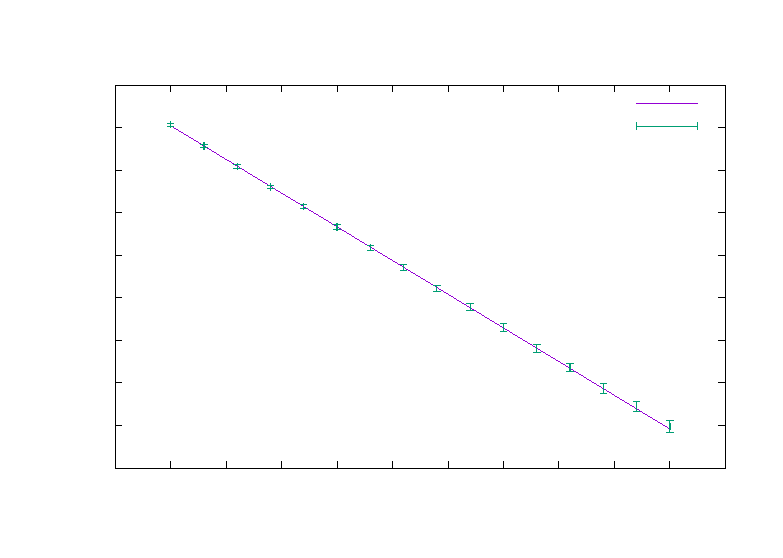
\includegraphics{tv3-plot}}%
    \gplfronttext
  \end{picture}%
\endgroup

		\caption{\centering Strömung des Wassers durch eine Kapillare \captionbr $\chi^2_{\text{red}} = 0.0946142 < 1 \implies$ Gute Kurvenanpassung\vspace{-1em}}
		\label{fig:tvthree-plot}
	\end{figure}

	Wir haben als Endergebnis:
    \begin{center}
        \begin{tabular}{l l}
            \toprule
            $\alpha$ & $\SI{-0.00158466(390)}{\per\second}$ \\
            $\beta$ & $\SI{5.80951(128)}{}$ \\
            \bottomrule
        \end{tabular}
    \end{center}
    \vspace{0.5em}
    Die $y$-Achsenabschnitt $\beta = \SI{5.80951(128)}{} = \SI{5.81(13)}{}$ laut der Kurvenanpassung stimmt mit dem gemessenen Wert $\ln\left[\left(h - h_\infty\right)\right]_{\text{exp}} = \SI{5.814(7)}{}$ überein.

    Nach Gleichung \eqref{eqn:tv3main} ist $\alpha$ und folglich die Viskosität von Wasser $\eta$ gegeben durch:
    \begin{equation}
    	\alpha = -\frac{\pi r^4 \rho g}{8\eta L A_v} \iff \eta = -\frac{\pi r^4 \rho g}{8\alpha L A_v} = -\frac{\cancel{\pi} d^4 \rho g}{128\alpha L \left(\cancel{\pi} r_v^2\right)} = -\frac{d^4 \rho g}{32\alpha L d_v^2} = -\left(\frac{\rho g}{32}\right) d^4\alpha^{-1}L^{-1}d_v^{-2}
    \end{equation}
    wobei $d =$ Durchmesser der Kapillare und $d_v =$ der Durchmesser des Vorratsrohres.
    
    Der Fehler $\Delta \eta$ ist dann:
    \begin{align}
    	\Delta \eta &= \gausserror{\eta}{d, \alpha, L, d_v} \notag \\
    	\text{\scriptsize (AMW Seite 20)} &=  \eta \times \sqrt{\left(4\frac{\Delta d}{d}\right)^2 + \left(\frac{\Delta \alpha}{\alpha}\right)^2 + \left(\frac{\Delta L}{L}\right)^2 + \left(2\frac{\Delta d_v}{d_v}\right)^2} \label{eqn:deltaEta}
    \end{align}

    Mit der folgenden Werten:
    \begin{center}
        \begin{tabular}{lrl}
            \toprule
            Variable & Wert & Bedeutung \\
            \midrule
            $g$ & \SI{9807}{\milli\meter\per\second\squared} & Erdfeldbeschleunigung \\
            $\rho$ & \SI{9.98e-4}{\gram\per\milli\meter\cubed} & Wasserdichte \\
            $\alpha$ & \SI{-0.00158466(390)}{\per\second} & Gefundene Steigung der Gerade \\ 
            $d$ & \SI{0.80(5)}{\milli\meter} & Durchmesser der Kapillare \\
            $d_v$ & \SI{15.95(5)}{\milli\meter} & Durchmesser des Vorratsrohres \\
            $L$ & \SI{245(4)}{\milli\meter} & Länge der Kapillare \\
            \bottomrule
        \end{tabular}
    \end{center}
    lässt sich $\eta$ und $\Delta \eta$ bestimmen:

    \begin{align}
    	\eta &= -\frac{\pbrace{\SI{0.80}{\milli\meter}}^4 \pbrace{\SI{9.98e-4}{\gram\per\milli\meter\cubed}} \pbrace{\SI{9807}{\milli\meter\per\second\squared}}}{32\pbrace{\SI{-0.00158466}{\per\second}} \pbrace{\SI{245}{\milli\meter}} \pbrace{\SI{15.95}{\milli\meter}}^2} \notag \\
    	&= \SI{1.26839e-3}{\gram\per\milli\meter\per\second} \sigfig{6} \\
    	\Delta \eta &= \pbrace{\SI{1.26839e-3}{\gram\per\milli\meter\per\second}}\\
    	&~~~\times\sqrt{\left(4\cdot\frac{\SI{0.05}{\milli\meter}}{\SI{0.80}{\milli\meter}}\right)^2 + \left(\frac{\SI{0.00000390}{\per\second}}{\SI{0.00158466}{\per\second}}\right)^2 + \left(\frac{\SI{4}{\milli\meter}}{\SI{245}{\milli\meter}}\right)^2 + \left(2\cdot\frac{\SI{0.05}{\milli\meter}}{\SI{15.95}{\milli\meter}}\right)^2} \notag \\
    	&= \SI{3.18e-4}{\gram\per\milli\meter\per\second} \sigfig{3}
    \end{align}
    Daraus folgt: $\eta_w = \eta = \SI{1.3(4)e-3}{\gram\per\milli\meter\per\second} = \SI{1.3(4)}{\milli\pascal\second}$

    Gefunden sei die Temperatur des Wassers $T = \SI{21.10(5)}{\celsius}$. Der Literaturwert $\eta_{w\text{~(lit)}} = \SI{0.978}{\milli\pascal\second}$ bei $\SI{21}{\celsius}$ liegt im Fehlerintervall des Wertes $\eta_{w\text{~(exp)}} = \SI{1.3(4)}{\milli\pascal\second}$. Diese zwei Werte stimmen miteinander überein.

